\documentclass[]{article}

\usepackage[left=2.00cm, right=2.00cm, top=2.00cm, bottom=2.00cm]{geometry}
\usepackage[spanish,es-noshorthands]{babel}
\usepackage[utf8]{inputenc} % para tildes y ñ

%opening
\title{Práctica 4. Exploración de grafos}
\author{Juan Carlos Lucena Monje \\ % mantenga las dos barras al final de la línea y este comentario
juancarlos.lucenamonje@alum.uca.es \\ % mantenga las dos barras al final de la línea y este comentario
Teléfono: 637929532 \\ % mantenga las dos barras al final de la linea y este comentario
NIF: 45899713q \\ % mantenga las dos barras al final de la línea y este comentario
}


\begin{document}

\maketitle

%\begin{abstract}
%\end{abstract}

% Ejemplo de ecuación a trozos
%
%$f(i,j)=\left\{ 
%  \begin{array}{lcr}
%      i + j & si & i < j \\ % caso 1
%      i + 7 & si & i = 1 \\ % caso 2
%      2 & si & i \geq j     % caso 3
%  \end{array}
%\right.$

\begin{enumerate}
\item Comente el funcionamiento del algoritmo y describa las estructuras necesarias para llevar a cabo su implementación.

Calculo el valor en funcion de la distancia a la que este de los obstaculos. Utilizo un incrementador para clasificar las distancias, consiguiendo que a mayor distancia haya menos valor tendra.

% Elimine los símbolos de tanto por ciento para descomentar las siguientes instrucciones e incluir una imagen en su respuesta. La mejor ubicación de la imagen será determinada por el compilador de Latex. No tiene por qué situarse a continuación en el fichero en formato pdf resultante.
\begin{figure}
\centering
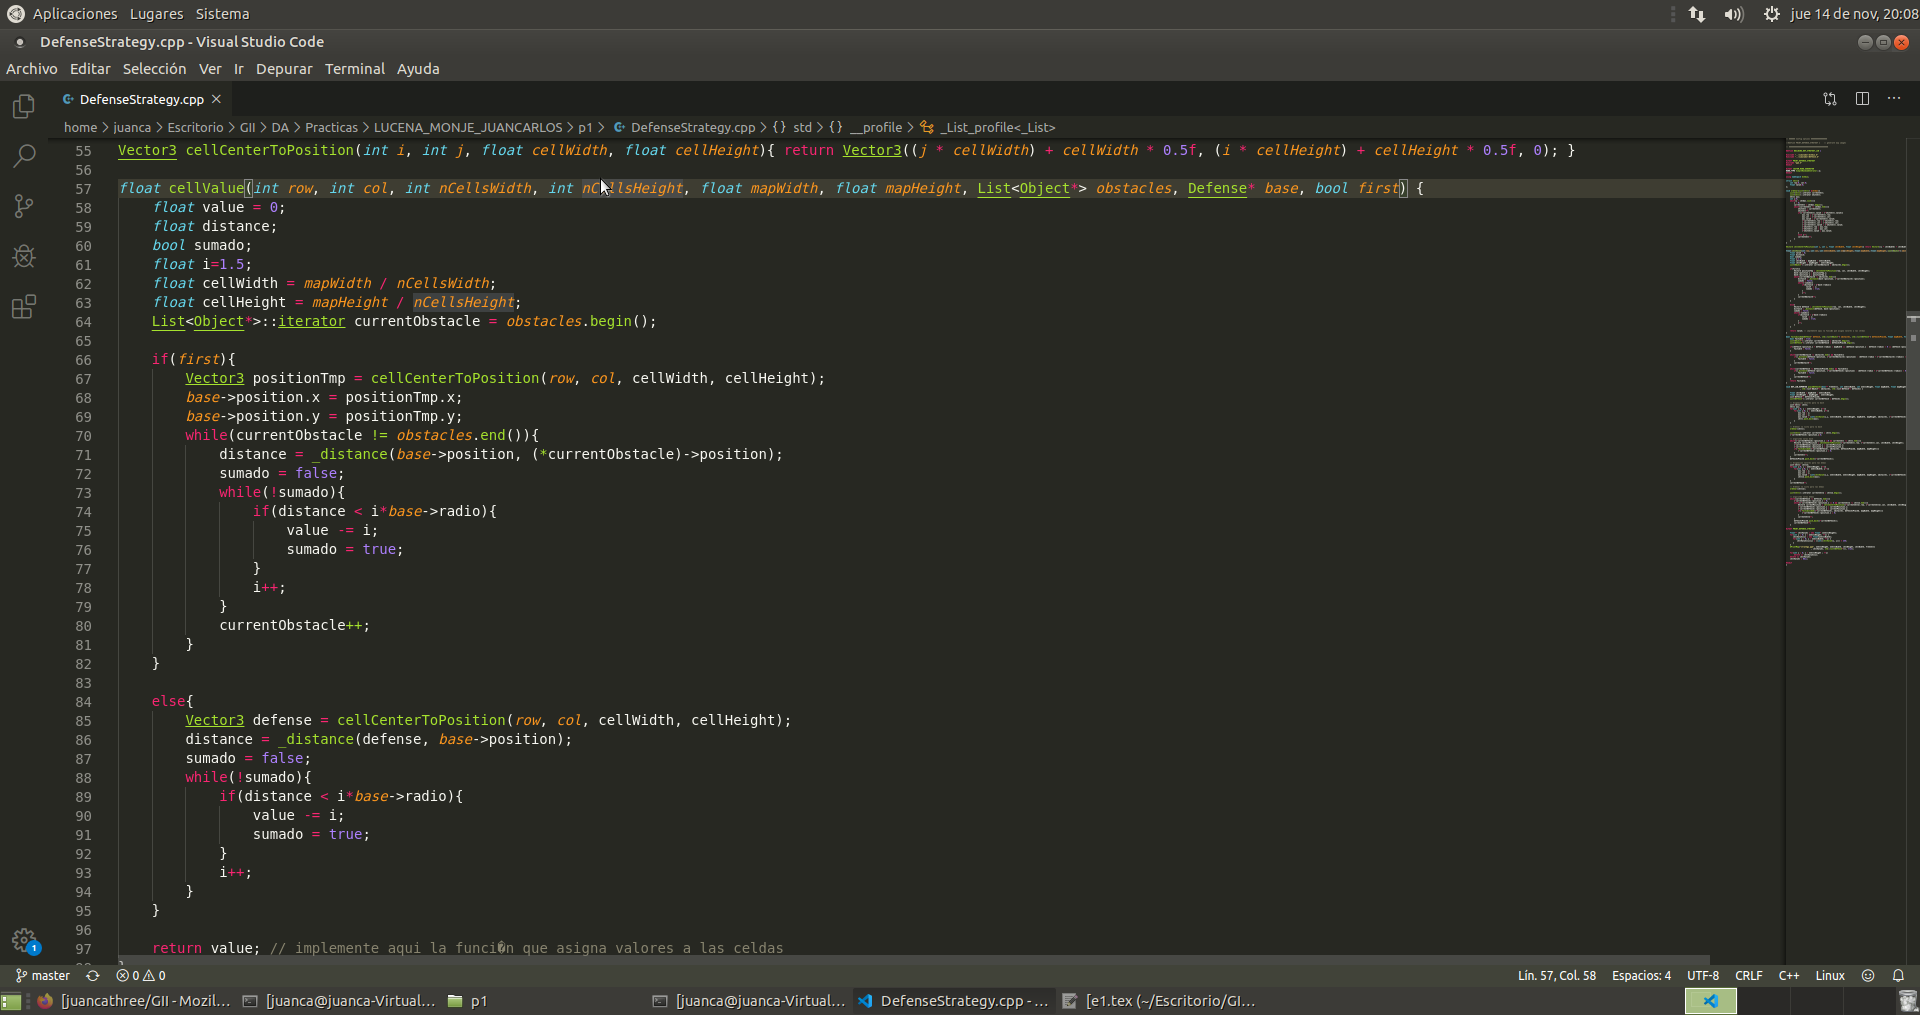
\includegraphics[width=0.7\linewidth]{./defenseValueCellsHead} % no es necesario especificar la extensión del archivo que contiene la imagen
\caption{Estrategia devoradora para la mina}
\label{fig:defenseValueCellsHead}
\end{figure}


\item Incluya a continuación el código fuente relevante del algoritmo.

Escriba aquí su respuesta al ejercicio 2.


\end{enumerate}

Todo el material incluido en esta memoria y en los ficheros asociados es de mi autoría o ha sido facilitado por los profesores de la asignatura. Haciendo entrega de esta práctica confirmo que he leído la normativa de la asignatura, incluido el punto que respecta al uso de material no original.

\end{document}
